\documentclass[a4paper,10pt,twoside,openany]{book}

\usepackage[lang=hebrew]{maths}
\usepackage{polynom}
\usepackage{hebrewdoc}
\usepackage{stylish}
\usepackage{lipsum}
\let\bs\blacksquare

\renewcommand{\Mat}{\mathrm{M}}

\setlength{\parindent}{0pt}

%%%%%%%%%%%%
% Styling %
%%%%%%%%%%%%

\usepackage{enumitem}

%%%%%%%%%%%%%
% Counters  %
%%%%%%%%%%%%%

\setcounter{section}{1}     

%%%%%%%%%%%%%%%%%%%%%%%%%%%%%%%%%
% Boxes around matrix elements  %
%%%%%%%%%%%%%%%%%%%%%%%%%%%%%%%%%
\usepackage{tikz}
\usetikzlibrary{matrix,fit}
\pgfkeys{tikz/mymatrix/.style={matrix of math nodes,inner sep=0pt,row sep=0em,column sep=0em,nodes={inner sep=6pt}}}

\newcommand*\mymatrixbox[5][]{\node [fit= (m-#2-#3) (m-#4-#5)] [draw=blue,thick,dashed,rounded corners,inner sep=-2pt,#1] {};}            

\newcommand{\highlightcells}[2][]{%
  \foreach \r/\c in {#2} {%
    \mymatrixbox[#1]{\r}{\c}{\r}{\c}%
  }%
}
            
%BIBLIOGRAPHY
\usepackage[
backend=biber,
style=alphabetic,
]{biblatex}
\addbibresource{bibliography.bib} %Imports bibliography file

\title{
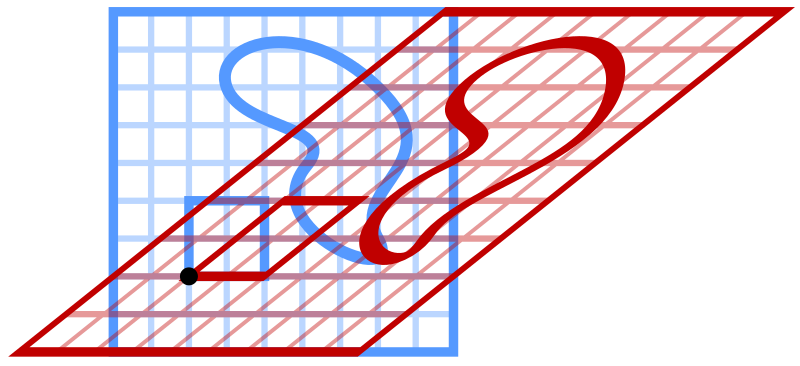
\includegraphics[width=6in]{images/front.png}\\
\vspace{30pt}
\Huge
אלגברה ב' (01040168)
\\
חורף 2026-2027
\\
רשימות תרגולים
\vspace{30pt}
\\
\huge
אלן סורני-רוזט
\vspace{30pt}
\\
\Large
הרשימות עודכנו לאחרונה בתאריך ה־%
\today
}
\date{}

\begin{document}
\frontmatter
\maketitle
\tableofcontents

\mainmatter

\section*{סימונים}

\begin{itemize}
\item[-]
$\brs{n} = \set{1, \ldots, n}$.
\item[-]
$\sum_{i \in \brs{n}} a_i = \sum_{i=1}^n a_i = a_1 + a_2 + \ldots + a_n$
\item[-] $\Mat_{m \times n}\prs{\mbb{F}}$ הוא מרחב המטריצות עם
$m$
שורות ו־%
$n$
עמודות, עם מקדמים בשדה
$\mbb{F}$.
\item[-]
$\mbb{F}^n = \Mat_{n \times 1}\prs{\mbb{F}}$
\item[-]
$\Mat_{n}\prs{\mbb{F}} = \Mat_{n \times n}\prs{\mbb{F}}$
\item[-]
$\hom_{\mbb{F}}\prs{V,W}$
הוא מרחב ההעתקות הלינאריות
$V \to W$
כאשר
$V,W$
מרחבים וקטוריים מעל
$\mbb{F}$.
\item[-]
$\End_{\mbb{F}}\prs{V} = \hom_{\mbb{F}}\prs{V,V}$
\item[-]
אותיות בפונט
\textenglish{mathcal}
עבור בסיסים -
$\mcal{B}, \mcal{C}, \mcal{D}$
וכו'
\end{itemize}

\part{חזרה}

\part{מרחבי מכפלה פנימית}

\part{צורת ז'ורדן}

\part{אלגברה מולטילינארית}

\printbibliography
\end{document}
